\documentclass{beamer}
\usepackage{lmodern}
\usepackage{HECbeamer} 
% \usepackage{pgfpages}
% \pgfpagesuselayout{4 on 1}[letterpaper, landscape, border shrink=5mm]
\title[\color{white}{MATH60604A Coefficient of determination}]{\texorpdfstring{MATH60604A \\Statistical modelling \\ \S 2e - Coefficient of determination}{MATH60604A \\Statistical modelling \\ \S~2e - Coefficient of determination}}
\author{Léo Belzile}
\institute{HEC Montréal\\
Department of Decision Sciences}
\date{} 
% \newcommand{\AIC}{\ensuremath{\mathsf{AIC}}}
% \newcommand{\BIC}{\ensuremath{\mathsf{BIC}}}
\begin{document}
\frame{\titlepage}

\section{Coefficient of determination}
% 
% \begin{frame}
% \frametitle{Review of linear regression }
%  Using the data $(\mathbf{X}, Y)$ from a sample, linear regression allows us to
% \bi
% 
% \item find the best fitting line/plane/hyperplane passing through the cloud of points,
% \item interpret the estimated linear trend (e.g., for each additional second spent fixating the ad, intention to buy increases on average by \ldots),
% \item judge how well the model explains the variability of the response.
% \ei
% To answer the last point, we need to review the concept of \textbf{linear correlation}.
% \end{frame}
% 




\begin{frame}
\frametitle{Pearson's linear correlation coefficient}
\bi
\item The correlation coefficient \alert{quantifies} the strength of the linear relationship between two random variables $X$ and $Y$. 
\item Suppose that we're studying $n$ pairs of observations $(X_1, Y_1),\ldots,(X_n, Y_n)$, where $(X_i, Y_i)$ are the values of $X$ and $Y$ for individual $i$.
\item Pearson's correlation coefficient is
\begin{align*}
R= \frac{\widehat{\mathsf{Co}}(X,Y)}{\sqrt{\widehat{\mathsf{Va}}(X)\widehat{\mathsf{Va}}(Y)}} = \frac{\sum_{i=1}^n (\mathrm{X}_i-\overline{X})(Y_i-\overline{Y})}{\sqrt{\sum_{i=1}^n(X_i-\overline{X})^2 \sum_{i=1}^n (Y_i-\overline{Y})^2}},\end{align*}
where $\overline{X}$ and $\overline{Y}$ are the sample means of $X$ and $Y$.
\ei
\end{frame}

\begin{frame}
\frametitle{Properties of Pearson's linear correlation coefficient}
\begin{tcolorbox}[colback=lightgray!30!white, colframe=lightgray!75!black, title=Properties of Pearson's linear correlation coefficient]
\bi
\item $-1 \leq r \leq 1$
\item $r=1$ ($r=-1$)  if and only if the $n$ observations fall exactly on a positively (negatively) sloped line. In other words, there exist two constants $a$ and $b > 0$ $(b <0$) such that $y_i=a+b x_i$ for any $i$.
\ei
\end{tcolorbox}
 \begin{center}
  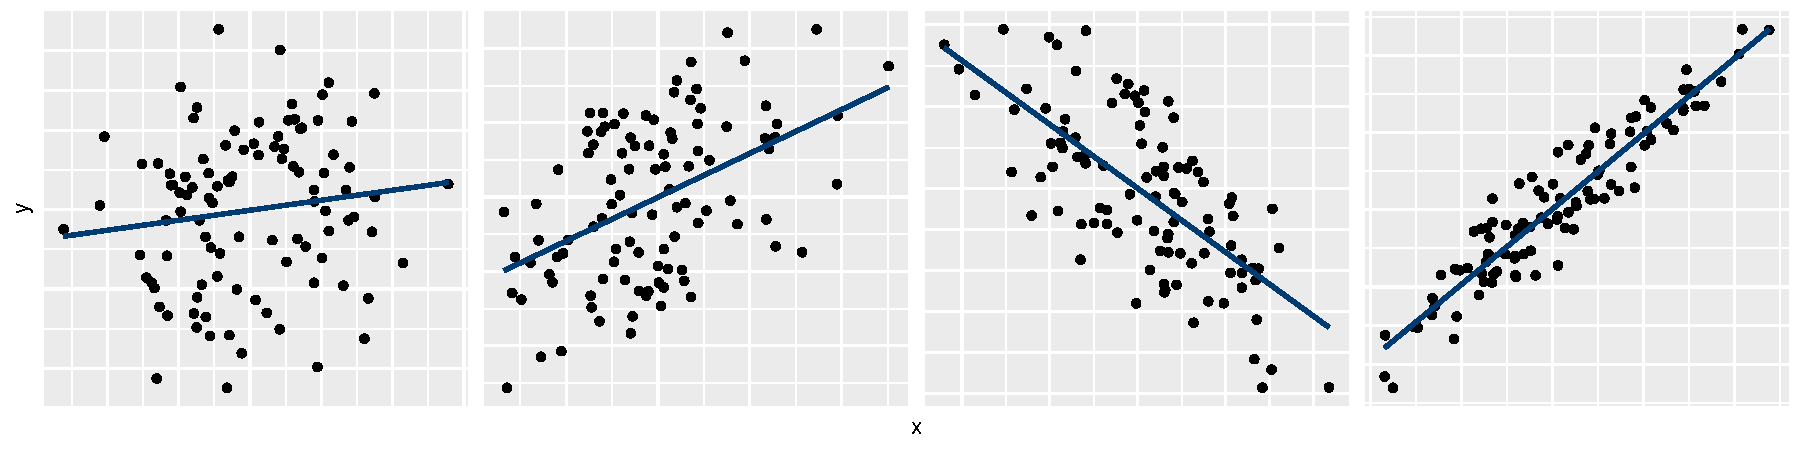
\includegraphics[width = \textwidth]{img/c2/03-linreg-correlation}
 \end{center}
{\footnotesize 
From left to right, the fours samples have linear correlation $0.1$, $0.5$, $-0.75$ and $0.95$. 


}
 
\end{frame}

\begin{frame}[fragile]
\frametitle{Pearson's linear correlation coefficient}
\bi
\item If $r>0$ ($r<0$), the two variables are positively (negatively) associated, meaning that $Y$ increases (decreases) on average with $X$.
\item The larger $|r|$, the less scattered the points are.

\item Independent variables are uncorrelated (not the other way around).
\item A correlation of zero does not imply that there is no relationship between the two variables.  It only means that there is no \textbf{linear} dependence between the two variables.

\ei

\begin{center}
 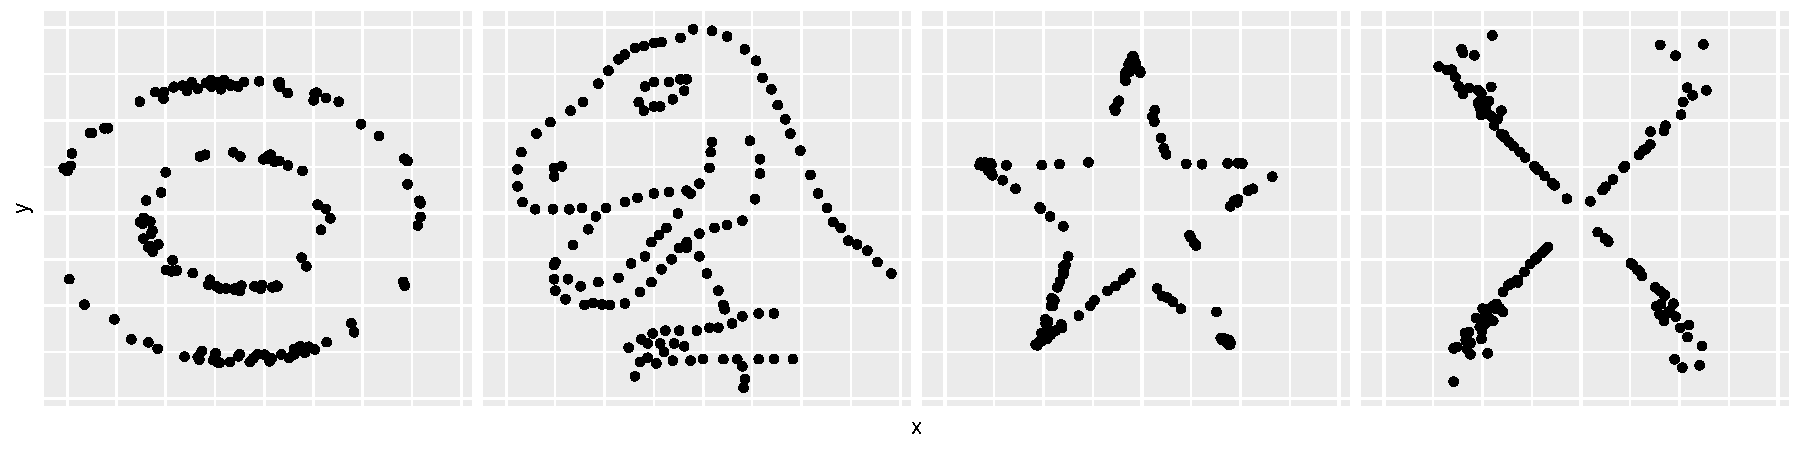
\includegraphics[width = 0.9\textwidth]{img/c2/03-linreg-datasaurus}
\end{center}
{\footnotesize
The four datasets (bullseye, Anscombosaurus, star, cross) have the same correlation of $-0.06$, yet the variables are clearly not independent.


}

\end{frame}
% \begin{frame}[fragile]
% \frametitle{  A picture is worth a thousand words}
% \begin{figure}
%  \centering
%  \includegraphics[width = 0.7\textwidth]{img/c2/Anscombe_quartet.pdf}
% \end{figure}
% Anscombe's quartet: each dataset has $r=0.82$.
% \end{frame}

% \begin{frame}
% \frametitle{Pearson's linear correlation coefficient}
% \bi
% \item \alert{\textbf{Caution:}} It can be misleading to interpret the correlation coefficient without examining the scatterplot.  A few examples in the next few pages will illustrate this.
% \item The following slides show scatterplots as well as the correlation coefficient in several situations where you'll have to use your own judgement.
% \item The last two examples show the dangers of interpreting the correlation coefficient without having examined the scatterplot.
% \ei
% \end{frame}
% 
%  \begin{frame}[fragile]
% \frametitle{Calculating the linear correlation in \SASlang}
% \begin{tcolorbox}[colback=white, colframe=hecblue, title=\SASlang code to calculate correlations]
% \begin{verbatim}
% proc corr data=infe.intention noprob;
% var intention fixation emotion;
% run;
% \end{verbatim}
% \end{tcolorbox}
% The linear correlation between \code{intention} and \code{fixation} is $0.43$ whereas the correlation between \code{emotion} and \code{intention} is about $0.23$.
% \end{frame}

\begin{frame}
\frametitle{Coefficient of determination}
\bi
\item Once the model has been fitted, it is be useful to have a measure that will tell us whether the model fits the data well.
\item The \alert{coefficient of determination}, $R^2$, measures the strength of the linear relationship between $\hat{Y}$ and $Y$.  
\item It is interpreted as the \alert{proportion of the variation} in $Y$ explained by the $\mathbf{X}$'s.
\item $R^2$ is the squared correlation between the predicted values and the response, $(\hat{Y}_1,Y_1),\ldots,(\hat{Y}_n,Y_n)$.
% \item We will now see its mathematical definition in the following slides.
\ei
\end{frame}

\begin{frame}
\frametitle{Sum of squares decomposition}
\bi
\item Suppose that we do not use any explanatory variable (i.e., the intercept-only model). In this case, the fitted value for $Y$ is the overall mean and the sum of squared centered observations
\begin{align*}
\mathsf{SS}_c=\sum_{i=1}^n (Y_i-\overline{Y})^2.
\end{align*}
\item When we include $\mathbf{X}$, the fitted value of $Y_i$ is rather $\widehat{Y}_i=\widehat{\beta}_0+\sum_{j=1}^p\widehat{\beta}_1 \mathrm{X}_{ij}$ and the sum of the squared residuals is
\begin{align*}
\mathsf{SS}_e=\sum_{i=1}^n (Y_i-\widehat{Y}_i)^2.
\end{align*}
\item The $\mathsf{SS}_e$ is non-increasing when we include more variables.
\ei
\end{frame}
% 
% \begin{frame}
% \frametitle{Sum of squares decomposition}
% \bi
% \item Define the sum of squared centered observations,
% \begin{align*}
% \mathsf{SS}_c=\sum_{i=1}^n (Y_i-\overline{Y})^2                                               \end{align*}
% 
% as the predicted value for each $Y_i$.
% \item When we include the $p$ regressors, the fitted value $Y_i$ is $\hat{Y}_i=\hat{\beta}_0+\hat{\beta}_1 \mathrm{X}_{i1}+\ldots+\hat{\beta}_p \mathrm{X}_{ip}$. Again, we define
% \begin{align*}
% \mathsf{SS}_e=\sum_{i=1}^n (Y_i-\hat{Y}_i)^2                                            \end{align*}
% as the sum of squared errors in the regression model including all the explanatory variables.

% \ei
% \end{frame}

\begin{frame}
\frametitle{Coefficient of determination ($R^2$)}
\bi
\item $R^2$ measures the  proportion of the variance in $Y$ explained by the set of predictor variables $\mathrm{X}_1, \ldots, \mathrm{X}_p$,
\begin{align*}
R^2=\frac{\mathsf{SS}_c-\mathsf{SS}_e}{\mathsf{SS}_c}.                                                     \end{align*}
\item When there is more than one explanatory variable, the square root of $R^2$ is also called the
\alert{multiple correlation coefficient}. 
\item $R^2$ always takes a value between $0$ and $1$.
\ei
\end{frame}

% \begin{frame}
% \frametitle{Coefficient of determination}
% \bi
% \item Recall that
% \bi
% 
% \item $\mathsf{SS}_c$ is the error for the intercept-only model
% \item $\mathsf{SS}_e$ is the sum of squared residuals of the model with the covariates $\mathbf{X}$. 
% \ei
% % \item Consequently, $\mathsf{SS}_c-\mathsf{SS}_e$ is the reduction of the error associated with including $\mathbf{X}$ in the model, or rather, the proportion of the variation in $Y$ explained by $\mathbf{X}$.
% \item By dividing by $\mathsf{SS}_c$, we end up with
% \begin{align*}
% R^2=\frac{\mathsf{SS}_c-\mathsf{SS}_e}{\mathsf{SS}_c}                                                     \end{align*}
% This gives the proportion of the variability in $Y$ explained by $\mathbf{X}$.
% \ei
% \end{frame}
% 
% \begin{frame}
% \frametitle{Properties of the coefficient of determination}
% \begin{tcolorbox}[colback=lightgray!30!white, colframe=lightgray!75!black, title=Properties of the coefficient of determination]
% \bi
% \item $0 \leq R^2 \leq 1$
% \item $R^2$ is the squared correlation coefficient between the fitted values $\hat{\bs{Y}}$ and the response $\bs{Y}$, i.e. the correlation of $(Y_1,\widehat{Y}_1),\ldots,(Y_n,\widehat{Y}_n)$
% \ei
% \end{tcolorbox}
% \end{frame}
% 
% 

 \begin{frame}
\frametitle{Coefficient of determination and interpretation}
\begin{center}
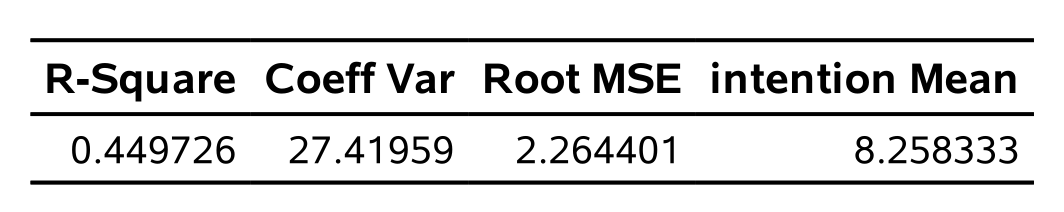
\includegraphics[width=0.6\linewidth]{img/c2/slides3-e13}
\end{center}
\bi
\item In the model with all of the explanatory variables,
$R^2=0.45$. Together, the explanatories explain $45\%$ of the variability in \code{intention}.
\item For the simple linear model with only \code{fixation} as covariate, 
$R^2 = 0.182$. That means the variable \code{fixation} explains $18.2$\%
of the variability in \code{intention}.
\ei
\end{frame}

 \begin{frame}
 \frametitle{A word of caution regarding $R^2$}
 \bi 
 \item 
 \textbf{Warning}: the more regressors you include in your model, the higher the $R^2$ (regardless of whether these variables are useful from an inference or predictive perspective).
  \item $R^2$ is therefore not a goodness-of-fit criterion.
  \item Software sometimes report the adjusted $R^2$,  which includes a penalty, \[R^2_a=1-(1-R^{2})\frac{n-1}{n-p-1}.\] The coefficient loses its interpretability and can be negative.
  \ei
  
  \end{frame}
  \end{document}
